\documentclass[12pt,a4paper]{article}

\usepackage[T1]{fontenc}
\usepackage[utf8]{inputenc} % Use UTF-8 encoding for input
\usepackage[french]{babel}

\usepackage{lmodern}	
\usepackage{amsmath}
\usepackage{amsfonts}
\usepackage{amssymb}
\usepackage{graphicx}
\usepackage{xcolor}
\usepackage{mathtools}
\usepackage{fancyhdr}
\usepackage{enumitem}
\usepackage{tcolorbox}
\usepackage{colortbl}
\usepackage{multirow}
\usepackage{stmaryrd}
\usepackage{dsfont}
\usepackage{tikz}
\usepackage{hyperref}
\usepackage{subcaption}
\usepackage[upgreek]{txgreeks}
\usepackage{algpseudocode}
\usepackage{algorithm}
\usepackage[text={15cm,24.5cm},centering]{geometry}


% Définir le texte affiché en fin de page
\pagestyle{fancy}
\fancyhf{}  % Clear the default headers and footers
\rfoot{\hrule
    \vspace{0.3cm}
    \noindent\textsf{Résolution de systèmes linéaires issus d'EDP}
    \hfill \thepage
}
\renewcommand{\headrulewidth}{0pt}

\title{\vspace{4cm}
        Rapport \\
        \vspace{1cm} \textbf{TP3 : Méthodes Multigrilles} \\ 
        \vspace{4cm} 
}

\author{\textit{Réalisé par} \vspace{0.5cm}\\
         \textbf{Mathilde Ferreira} \\
        \textbf{Félix Foucher de Brandois}
}
        
\date{\vfill
        \textit{ENSEEIHT} - 
        \textit{Formation ModIA, 5$^{e}$ année}
        \hfill
        \textit{2024-2025} \\
        \vspace{1cm}
}


\begin{document}

\begin{figure}[t]
    \centering
    
\includegraphics[width=7cm]{src/inp_n7.png}
    \hfill
    
\includegraphics[width=5.5cm]{src/insa_toulouse.png}
\end{figure}


\maketitle
\thispagestyle{empty}

\newpage


\section{Introduction}

L'objectif de ce TP était d'implémenter une méthode multigrilles de type V-cycle en 1D pour résoudre le problème de Poisson avec des conditions aux limites de Dirichlet homogènes.
Le problème est défini par l'équation différentielle suivante :
\begin{equation}
    \begin{cases}
        -u''(x) = f(x) & \text{sur } \Omega = [0, 1] \\
        u(0) = u(1) = 0
    \end{cases}
\end{equation}

Pour ce TP, nous avons choisi une solution analytique connue : $u(x) = x^2(1 - x)^2$, ce qui donne $f(x) = -u''(x) = -2 + 12x - 12x^2$. \\
La solution exacte satisfait naturellement les conditions aux limites.
Cette solution nous permet de calculer l'erreur de discrétisation et de valider notre implémentation.

Les parties suivantes couvrent la construction de la méthode multigrille, sa mise en œuvre via un schéma \textit{V-cycle}, l’analyse des résultats obtenus et enfin une comparaison avec un solveur direct.

\section{Méthode Multigrille (V-cycle)}

\subsection{Principe}
La méthode multigrille repose sur la combinaison de plusieurs niveaux de maillages pour accélérer la convergence vers la solution. Elle repose sur trois opérations principales :

\begin{itemize}
    \item \textbf{Relaxation} : souvent réalisée avec un schéma de Gauss-Seidel, elle réduit les composantes hautes fréquences de l'erreur.
    \item \textbf{Restriction} : transfert du résidu vers un maillage plus grossier.
    \item \textbf{Prolongation} : interpolation des corrections obtenues sur le maillage grossier vers le maillage fin.
\end{itemize}

\subsection{V-cycle}
Le \textit{V-cycle} applique successivement ces opérations, permettant une réduction efficace des différentes composantes de l’erreur. Une seule itération du V-cycle peut suffire à fortement réduire l’erreur globale, surtout si elle est combinée à des phases de relaxation avant et après correction.

\section{Résultats pour différentes tailles de maillage}

\subsection{Évolution du résidu}
La figure suivante montre l'évolution du résidu en fonction du nombre d'itérations pour différentes tailles de maillage $N$ :

\begin{figure}[H]
    \centering
    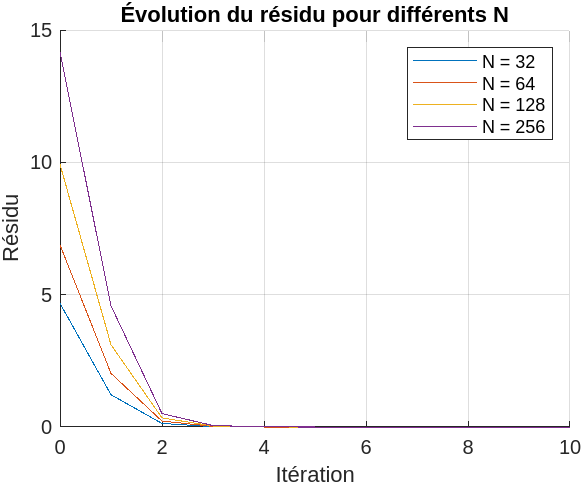
\includegraphics[width=0.8\textwidth]{src/res.png}
    \caption{Évolution du résidu pour différentes tailles de maillage $N$.}
\end{figure}

\textbf{Analyse :} on constate une décroissance rapide du résidu dès les premières itérations, quel que soit le maillage utilisé. Cette convergence rapide est caractéristique du V-cycle multigrille, capable de réduire efficacement les erreurs à toutes les échelles.

\subsection{Erreur de discrétisation}
La figure ci-dessous montre l'évolution de l'erreur en norme $L^2$ au cours des itérations.

\begin{figure}[H]
    \centering
    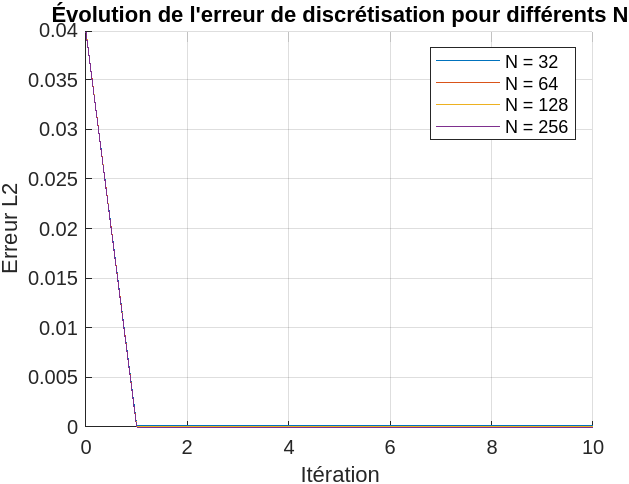
\includegraphics[width=0.8\textwidth]{src/L2.png}
    \caption{Évolution de l'erreur de discrétisation $L^2$ pour différentes tailles de maillage $N$.}
\end{figure}

\textbf{Analyse :} l’erreur devient quasi nulle dès les premières itérations. Cela signifie que le multigrid converge non seulement rapidement en termes de résidu, mais aussi en termes de solution approchée.

\subsection{Erreur finale en norme $L^2$}

\begin{table}[H]
\centering
\begin{tabular}{|c|c|c|}
\hline
\rowcolor{gray!20} \textbf{Taille $N$} & \textbf{Erreur L2 finale} & \textbf{Ratio erreur$_N$ / erreur$_{2N}$} \\
\hline
32  & 1.7830e-04 & 4.00 \\
64  & 4.4574e-05 & 4.00 \\
128 & 1.1143e-05 & 4.00 \\
256 & 2.7859e-06 & - \\
\hline
\end{tabular}
\caption{Erreur de discrétisation $L^2$ finale pour différentes tailles de maillage $N$, avec le ratio entre deux tailles consécutives.}
\end{table}

\textbf{Interprétation :} le ratio d’erreur est très proche de 4, ce qui est cohérent avec un schéma de discrétisation d’ordre 2 : on observe bien une décroissance quadratique de l’erreur quand on affine le maillage.

\subsection{From 2-grid to multigrid}

\subsubsection*{Objectif}
Dans cette étape, on généralise le V-cycle à un algorithme multi-niveaux (\(L+1\) niveaux), en modifiant la fonction \texttt{V\_cycle.m} en une version récursive \texttt{V\_cycle\_L.m} acceptant un paramètre $L$ représentant le nombre de niveaux de maillage.

\subsubsection*{Réflexion préalable}
\begin{enumerate}
    \item \textbf{Quelle partie de l’algorithme doit être modifiée ?}\\
    La principale modification concerne l'étape de résolution sur le maillage grossier. Plutôt que de résoudre directement le problème à ce niveau, si l’on n’a pas encore atteint le niveau le plus grossier, on appelle récursivement le V-cycle sur un niveau plus bas.

    \item \textbf{Pourquoi utiliser plus de deux niveaux ?}\\
    Ajouter davantage de niveaux permet de réduire encore plus rapidement les composantes basses fréquences de l’erreur. Cela améliore l’efficacité du solveur, en particulier pour les grands maillages, car la résolution sur les niveaux grossiers est peu coûteuse et permet de propager des corrections efficaces à grande échelle.
\end{enumerate}

\subsubsection*{Expérience numérique}

\textbf{Conditions :} Maillage fixé à \(N = 256\), variation du nombre de niveaux \(L\) dans l’algorithme \texttt{V\_cycle\_L.m}.

\begin{itemize}
    \item \textbf{1. Quel est le niveau \(L\) maximal utilisable ?}\\
    Le niveau \(L\) maximal correspond au plus petit maillage possible contenant encore des points internes. Pour un maillage 2D de taille N=$2^k$, si l’on divise par 2 à chaque fois, on ne peut pas aller au-delà d’un maillage de taille \(N = 2\) car ensuite il ne resterait que les bords. On aurait donc \(L = k-1\) (avec \(k-1\) niveaux au total).

    \item \textbf{2. Obtient-on la même erreur de discrétisation qu’avec la méthode à deux niveaux ?}\\
    Oui, les tests effectués montrent que l'erreur de discrétisation finale (en norme $L^2$) reste identique quelle que soit la profondeur du multigrid (tant que l’on ne change pas le maillage \(N\)). En effet, la méthode converge vers la même solution discrète. Ce sont uniquement les performances qui changent.

    \item \textbf{3. Que remarque-t-on sur la réduction d’erreur ?}\\
    On observe que plus on augmente le nombre de niveaux \(L\), plus la convergence est rapide. Cela s’explique par le fait que l’erreur basse fréquence est corrigée plus efficacement lorsqu’elle est transmise à des niveaux de maillage très grossiers. Ainsi, l’ajout de niveaux accélère la décroissance du résidu et du nombre d’itérations nécessaires.
\end{itemize}

\textbf{Conclusion :} L’introduction d’un algorithme multigrille à plusieurs niveaux permet d’améliorer considérablement les performances de convergence, tout en conservant la précision de la méthode 2-grid. Cela constitue une étape importante avant de passer à la méthode \textit{Full Multigrid} (FMG).
\end{document}